\documentclass[pra,aps,showpacs,groupedaddress,superscriptaddress,twocolumn,toc=flat]{revtex4-1}

\usepackage[colorlinks=true,linkcolor=blue,urlcolor=blue,citecolor=blue]{hyperref}

\usepackage[utf8x]{inputenc}
\usepackage{color}
\usepackage{bbm} 

\usepackage{amsfonts,amsmath,amssymb,stmaryrd}

\usepackage{graphicx}
\usepackage{subfigure}  % use for side-by-side figures
\usepackage{bbm} 
\usepackage{hyperref}
\usepackage{epsfig}
\usepackage{mathrsfs}
\usepackage{verbatim}
\usepackage{centernot}
\usepackage{ulem}
\usepackage{longtable}
\usepackage{nicefrac}
\usepackage[framemethod=tikz]{mdframed}

\begin{document}

\title{Tutorial on the Bose-Hubbard model}

\begin{abstract}
In this tutorial we analyze the three phases of the Bose-Hubbard model on the square lattice, namely the superfluid phase, the Mott insulator, and the normal gas.
We will set up the corresponding initial files, let the code run till we reach error bars at the percent level, and compare various quantities such as the superfluid density, the density profile, the density matrix, and the compressibility.


\end{abstract}

\maketitle

\section{Compiling the code}
We assume that the reader has already been able to successfully compile the code before, and is familiar with the Monte Carlo examples and tutorials provided by ALPSCore.
In the \texttt{cmake} variables  we make sure that the lattice variable is set to \texttt{square}, the variable \texttt{CWINDOW} is switched \texttt{OFF}, and \texttt{UNIFORM} must be on. 
On \texttt{Linux} operating systems we can achieve this by going to the \texttt{build} directory, typing \texttt{ccmake .} and edit the corresponding variables. We are now in a position to recompile the code.
The simplest way to go through the tutorial is to copy and edit the parameter files provided in the \texttt{parameterfiles} directory. We set  \texttt{Lx = Ly = 8}, and work with periodic boundary conditions, \texttt{pbcx = pbcy =1}.
Our energy unit is set by taking unity for the hopping amplitude,  \texttt{$t_{hop} = 1.0$}, and we look at on-site interactions only, \texttt{$V_{nn} = 0.0$}.

\section{The normal gas}
The system will always be in the normal phase when temperature is high enough. There are no long-range correlations, no superfluidity, but the gas is compressible. In the world-line picture,
particles correspond to nearly-straight, slightly wiggling worldlines in imaginary time, with few quantum fluctuations due to hopping terms in the Hamiltonian. If we set $U_{on} = 8$, $\mu = 3$ and $\beta = 0.2$ then we are in the desired regime. As we expect that the worm algorithm behaves no different than just local updates, we should increase the program variables  \texttt{Nmeasure} and  \texttt{Nmeasure2} substantially to $L_x \times L_y$ and $(L_x \times L_y)^2$, respectively, which are sensible choices. Setting the number of sweeps to $10^7$ gives good enough statistics for our purposes, and should take only a few minutes on a single processor. Better statistics can be obtained by running longer. \\

Analyzing the output, we see that the variance in total particle number, $\left< N^2 \right> - \left< N \right>^2$, is greater than zero. There are hence substantial fluctuations in particle number, as we expect for a compressible phase. The superfluid density is (almost) zero; the very small values seen in the winding numbers along $x$ and $y$ are a finite size effect.  The equal-time density matrix shows exponential decay (if one takes a bigger system size, then this is easier to see). 


\section{The superfluid phase}
The system enters the superfluid phase at low enough temperature. For non-commensurate densities this occurs for any value of $U_{on}$, while for commensurate densities $U_{on}$ must be sufficiently small. For unit density, the critical value is $U_c \approx 16.74$ in the ground state. 
The transition between the normal phase and the superfluid phase as a function of temperature is of the Kosterlitz-Thouless type. This implies that the condensate fraction remains zero and that the equal-time density matrix decays algebraically with distance at any finite temperature and for a big enough system size. This is a consequence of the Mermin-Hohenberg-Wagner theorem that states that a continuous symmetry cannot be broken spontaneously in two and lower dimensions. In the ground state ($T = 0$) however, condensation can take place, and the equal-time density matrix approaches a constant for long enough distances. Note that near-constant behavior can also be seen for finite system sizes at low but finite temperature.  A superfluid phase is furthermore compressible. Setting $U_{on} = 8$, $\mu = 12$ and $\beta = 1$ we are going to find the target behavior. As we expect that the worm algorithm will visit most of the system volume in a single sweep, we can set \texttt{Nmeasure} equal to 1. If we choose $10^5$ sweeps, then we get an accuracy of $3-4\%$ within a few minutes on a single core. \\

Analyzing the output, we see that the variance in total particle number, $\left< N^2 \right> - \left< N \right>^2$, is greater than zero. There are hence substantial fluctuations in particle number, as we expect for a compressible phase. 
The winding number fluctuations are very large, indicating a very large superfluid density. Finally the  equal-time density matrix behaves as described above.


\section{The Mott insulator}
The Mott insulator is reached when the density is commensurate, and the interaction strength strong enough. It is a gapped, insulating and incompressible phase, where the density is pinned to an integer value.
Setting $U_{on} = 30$, $\mu = 12$ and $\beta = 5$ we are going to see the desired behavior for $n=1$. Strictly speaking, the Mott insulator only exists at zero temperature. There is however a gap $\Delta$ which is $ \Delta \sim U$ deep enough in the insulating phase. Hence, for $T \ll \Delta$, we are very close to the ground state.  As for the normal phase, we expect that the worm algorithm behaves no different than just local updates. We should hence increase the program variables  \texttt{Nmeasure} and  \texttt{Nmeasure2} substantially to $L_x \times L_y$ and $(L_x \times L_y)^2$, respectively. \\

Analyzing the output, we see that the variance in total particle number, $\left< N^2 \right> - \left< N \right>^2$ is (very close to) zero. There are hence no fluctuations in particle number, as we expect for an incompressible phase. The superfluid density is (almost) zero; the very small values seen in the winding numbers along $x$ and $y$ are a finite size effect.  The equal-time density matrix shows exponential decay (if one takes a bigger system size, then this is easier to see). The density profile is exactly one, within error bars, on every site. Note however, that the expectation value of the kinetic energy is nonzero, {\it i.e.}, there are some quantum fluctuations left, and the ground state is not a product state. \\


In Fig.~\ref{fig:dm} we show the equal time density matrix for the three phases along the $x$-axis for the parameter values specified above. The symmetry in the curves is a consequence of the periodic boundary conditions. One further clearly sees the exponential decay for the normal gas and Mott insulating phases, and the power-law decay in the superfluid phase. The reader is welcome to repeat the above analysis for bigger systems sizes (and longer runtimes). 


\begin{figure}[h!]
\centering
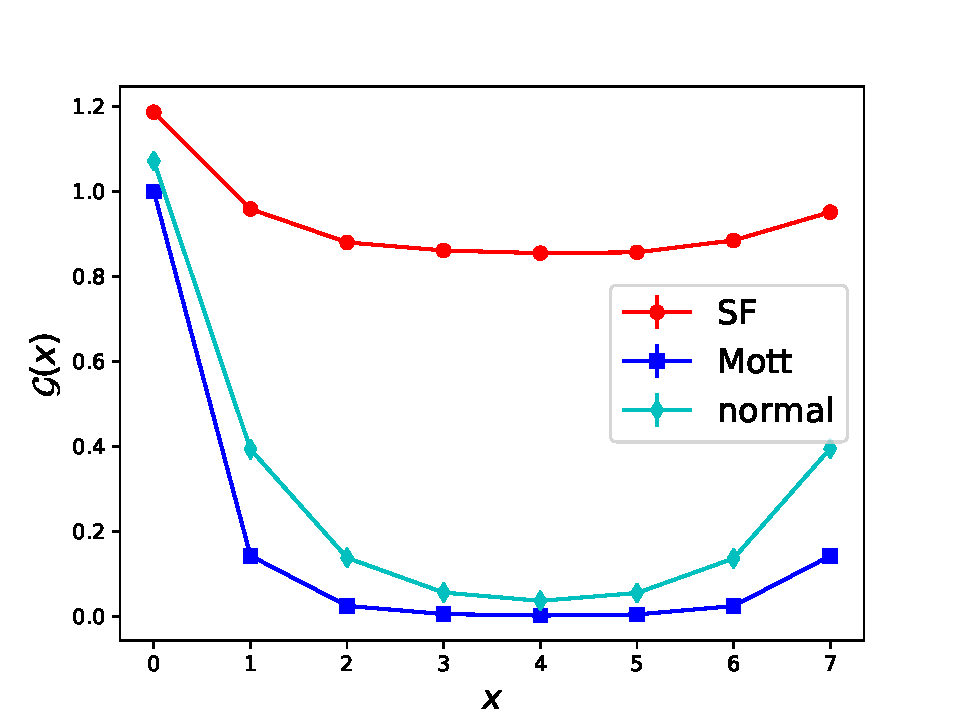
\includegraphics[width=0.6\linewidth]{fig_density_matrix.pdf}
\caption{Equal time density matrix along the $x$-axis in the three phases, superfluid (SF), Mott insulator (Mott), and normal gas (normal), for the parameters mentioned in this tutorial. } 
\label{fig:dm}
\end{figure}




\end{document}
